\documentclass{acm_proc_article-sp}

\usepackage{algorithm}
\usepackage{algorithmic}

\begin{document}

\title{Addressing Redistribution in Bikeshare Using Cox Processes and Online Supervised Learning}

\numberofauthors{1}
\author{
\alignauthor
Walter Dempsey\\
       \affaddr{University of Chicago}\\
       \affaddr{5734 S. University Avenue}\\
       \affaddr{Chicago, IL}\\
       \email{wdempsey@galton.uchicago.edu}
}

\maketitle

\begin{abstract}
A bicycle sharing system (bikeshare) is a service in which individuals can check-out bicycles from stations for a short period of time and drop them off at any of the stations in the system. The main purpose of bikeshare is to provide transportation for short trips, and it has become common in many cities including New York, Paris, and Beijing. One of the issues with bikeshare is the possible imbalance of bikes across stations, specifically that some stations may have no bikes to check-out while other stations have no slots for arriving bikes. Many cities employ re-distribution techniques on an ad hoc basis. In order to improve the redistribution process, we must estimate the expected number of bikes at a station at some point in the future, as well as the chance that the station becomes empty or full in that time window. To do this, we model the arrival and departure of bikes as a log Gaussian Cox Process. We build a block approximation of the underlying Gaussian processes by clustering  neighborhoods, which will allow for parallel estimation. Moreover, we build online methods for updating the parameters from streaming station data. In order to assess performance, we apply these techniques to the Washington D.C. bikeshare data. We end with a brief discussion of how our approach can be used in analyzing new stations without sufficient data and as well as new networks/cities. 
\end{abstract}


\terms{Log Gaussian Cox Processes, Block-Approximate Gaussian Processes, Parallel Algorithms, Online Learning}

\section{Introduction}

Bicycle Sharing systems have become ubiqutious over the past several years, providing an alternative mode of transportation and improving the connectivity of their respective cities.  These networks (typically referred to as bikeshare) consist of a number of stations distributed throughout the city with individuals able to check-out bicycles from stations for a short period of time before dropping them off at another station in the system.  A common issue with bikeshare is that traffic patterns commonly result in bike imbalance across stations, with some stations being either empty or full.  We call these {\bf extreme} stations.  This leads to delays as bikeshare users must find alternate stations, while also lowering overall ridership due to reliability concerns. Bikeshare systems tackle this issue by some form of redistribution; however, the methods for redistribution of bikes is ad hoc and may be sub-optimal.

For a given time in the future, we wish to predict the number of bikes at the station as well as the probability of the station becoming extreme at some point in this time window given its current state as well as auxiliary variables.  This will allow us to predict extreme stations as well as provide an estimated optimal number of bikes per station during redistribution to avoid extreme events in the next time window.

We model arrival and departure of bikes at each station as a pair of correlated Poisson Processes.  We propose then modeling the entire bikeshare system as a set of correlated Poisson Processes, where two pairs are correlated based on their spatial proximity.  This set is therefore modeled as a log-Gaussian Cox Process in which we capture station-level, temporal, and spatial random effects.  

This approach is computationally intensive, and therefore we propose approximation methods for estimation, which allow us to run estimation in parallel and provide necessary speedups at the cost of some inexactness.  The bikeshare data analyzed is also streaming, and therefore we provide an online algorithm which updates parameter estimates given the new observations.  This allows us to update models given new data without re-fitting the entire model everytime.  We end with an application of our techniques to Washington D.C. bikeshare data.  We analyze the performance, and provide methods for prediction of new stations given estimation from surrounding stations.


\section{Arrival and Departure Processes}

We start by considering the temporal process at a given station.  Let $Y_i (t)$ denote the number of bikes at the station at time $t$.  The bike count is an integer-valued process with jumps.  We use $Y(t)$ to define a pair of counting processes which we then model.

The {\bf arrival counting process}, $N_i^{a} (t)$ can be defined as the number of bikes arriving at the station up to time~$t$.  Assuming a finite number of bike arrival times in any interval, we can then define these counting processes as:
\begin{align}
N^{a} (t) &= \sum_{s < t} \left | Y_i (s) - Y_i (s-) \right | {\bf 1} \left[ Y_i (s) - Y_i (s-)  > 0 \right] 
\end{align}
The {\bf departure counting process}, $N_i^{d} (t)$ can be defined likewise for bikes leaving the station.  A consideration is that a station which is empty cannot have departures.  Therefore, $Y_i (t) = 0$ in some interval~$[t, t+\delta]$ implies $N_i^{d} (t+\delta) -N_i^{d} (t) = 0$.   Let $A_{d}$ be the set of all such windows.  Then, we assume the departure counting process to be an inhomogenous Poisson point process on the complement of this set, $\mathbb{R}^{+} - A_{d}$.  We consider the same to be true of the arrival process and the window of all times for which the station is full, $A_{f}$.

For now, we ignore these constraints on the process.  We assume that at a station, the arrival and departure counting processes are correlated.  This implies that we can model the pair as a Cox process where the rate parameters includes a station block effect. That is, $N_i^(a) (t)$ ($N_i^{d} (t)$ respectively) are poisson processes with rate parameter $\lambda_i^{a} (t)$ ($\lambda_i^{d} (t)$ respectively) where
\begin{align}
\log \left( \lambda_i^{a} (t) \right) = \mu^{a}_i(t) + b_i
\end{align}
\noindent where $b_i$ is a random station effect.  The rate parameter for the departure process can be defined similarly.

\section{Bikeshare System}

We now consider the complete bikeshare system.  Stations in close geographic proximity provide auxiliary information which should be leveraged.  For example, if a station has many arrivals in a given morning, this is a strong indicator that the number of arrivals at a neighboring station will also be high.  We wish to introduce the spatial dependency into our current model.  

We use a log-Gaussian Cox Process to do this in which spatial dependence is captured through random effects in the stochastic rate parameters.  Let $N_i (t) = (N_i^(a) (t), N_i^{d} (t))$ be the pair of counting processes for station~$i$.  Then we can assume that the arrival rate parameters are associated as are the departure rate parameters.  So that
\begin{align}
\log \left( \lambda_i^{a} (t) \right) = \mu^{a}_i(t) + b_i + Z(t;i)
\end{align}
\noindent where $Z(t;i)$ is a mean-zero gaussian process with covariance that may depend on both time~$t$ and space~$i$.  We can incorporate the station effects into the gaussian process model.  We then consider a simple separable variance components model :
\begin{align*}
\text{cov} ( Z(t;i) , Z(t^\prime; j) ) =& \sigma_0^2 \delta_{t t^\prime}  \delta_{i j} + \sigma_1^2  \delta_{i j} \\
&+ \sigma_2^2 \exp \left( -\frac{ d(i,t),(j,t)) }{\lambda} \right)
\end{align*}
\noindent where $d ( (i,t) , (j,t))$ is a specified distance metric. In our work we consider the $l_2$ distance.  The first term is measurement error at time~$t$ at station~$i$, the second is the random station effect, and the third is a general mean associated with all the arrival parameters.

Covariates can be chosen to account for temporal trends.  We can choose a factor model for $\mu^{a})i (t)$ which would model fixed effects attributable to time of day, month, and year, or a basis expansion in terms of low-order Fourier terms.  In this case, the distance metric will only depend on the location of the stations and the third term will only be included when $t$ and $t^\prime$ are equal.

We assume a similar model for the departure rates.  The random block effects link the arrival and departure processes at a given station, and the third term in the gaussian process links the rate parameters for the arrival processes across stations.  The departure processes across stations are linked via a similar term, albeit different parameter values, $(\sigma_3^2, \lambda^\prime)$.

\section{Maximum Likelihood Estimation}

Suppose that there are $n$ total stations. Now take the observations at a particular time window, $(t , t+\delta)$ (we model half-hour windows).  The general form of the Cox Process Likelihood associated with the data, \\ $Y(t) = \left( (Y_1^{a} (t), Y_1^{d} (t)), \ldots, (Y_n^{a} (t), Y_n^{d} (t)) \right) $ is:
\begin{align*}
&l_t( \theta; Y(t) ) = \int_{\Lambda} P(X,  \Lambda | \theta) d \Lambda \\
&= \int\prod_{i=1}^n \frac{\lambda_i^{a} \lambda_i^{d}}{Y_i^{a} Y_i^{d}} \frac{e^{-\lambda_i^{d}-\lambda_i^{a} }}{(2 \pi)^{n} |\Sigma|^{1/2}} \exp \left( (\lambda - \mu (\theta) )^T \Sigma (\theta) ^{-1} (\lambda - \mu (\theta) ) \right) d \lambda \\
&= E_{\lambda | \theta} [l^{\star} ( \lambda; Y(t))]
\end{align*}
\noindent where $l^{\star} ( \lambda; Y)$ is the likelihood for the inhomogeneous Poisson process, and $\lambda$ is the vector of rate parameters for the dual processes at each station.  As we incorporate temporal trends through the the model for the mean, $\mu$, the complete likelihood is the sum over all time windows.  Supposing we have $T$ total time windows, $(t_1, \ldots, t_T)$, then the complete likelihood is:
\begin{align*}
l ( \theta; Y ) = \sum_{i=1}^T  E_{\lambda | \theta} [l^{\star} ( \lambda; Y (t_i)]
\end{align*}
In our setting, the likelihood for each time window consists of estimating an expectation over the finite-dimensional distribution of $\lambda$.  The number of stations is of the order of several hundred.  Washington D.C. has roughly $250$ stations, and therefore the dimension of our expectation is approximately $500$.  The high dimensionality of the integration appears formidable. 

\subsection{Monte Carlo Estimation} 
Standard Monte Carlo methods would employ the estimate:
\begin{equation}
l_{MC} (\theta) = s^{-1} \sum_{j=1}^s l \left( \theta | X, \lambda^{(j)} \right)
\end{equation}
\noindent where $\lambda^{(j)}$ are simulated realisations of $\lambda$.  This is highly inefficient.  Based on the work of Geyer (1999) and Diggle et al. (2013), we use the following to provide robust, efficient estimation of the log-likelihood function.  Given un-normalized joint density of $X$ and $\lambda$, $f(X, \lambda | \theta)$, then 
\begin{align}
\hat{L} \left( \theta \right) =& \log \big \{ s^{-1} \sum_{j=1}^s r \left( X , \lambda^{(j)} , \theta, \theta_0 \right) \big \} \label{approx_lik} \\
&- \log \big \{ s^{-1} \sum_{j=1}^s r \left( X^{(j)} , \lambda^{(j)} , \theta, \theta_0 \right) \big \} \notag
\end{align}
\noindent where $r(X, \lambda, \theta, \theta_0) = f(X, \lambda | \theta)/f(X, \lambda | \theta_0)$. The result provides a Monte Carlo approximation to the log-likelihood function, and consequently the maximum likelihood estimate, $\hat{\theta}$, by simulating the process at a single value, $\theta_0$.  The accuracy is a function of the number of simulations, $s$, and the proximity of $\theta_0$ to $\theta$.

The pair $(X^{(j)}, \lambda^{(j)})$ are simulated joint realisations of $X$ and $\lambda$ at $\theta = \theta_0$.  In the first term, $X$ is held fixed and $\lambda^{(j)}$ are conditional on $X$.  Conditional simulation of $\lambda$ requires Markov Chain Monte Carlo (MCMC) methods.  Design, computational issues, and design are detailed by Diggle et al. (2013).  Algorithm \ref{applik_alg} outlines pseudocode for finding the maximum likelihood estimate, $\hat{\theta}$.

\begin{algorithm}[!h]
\caption{Block-Approximate Cox Process} \label{applik_alg}
\begin{algorithmic}
\STATE {\bf ApproxCP}$(Y, s, \theta_0)$
\FOR{$j$ in $1:s$}
\STATE Generate $(\lambda^{(j)}, Y^{(j)})$ at $\theta = \theta_0$
\STATE Generate $\lambda_2^{(j)}$ given $Y$ at $\theta = \theta_0$ via MCMC
\ENDFOR
\STATE Estimate $\hat{L} (\theta)$ by equation~\eqref{approx_lik}
\STATE $\hat{\theta} \gets \arg \max \hat{L} (\theta)$ given $\theta_0$
\end{algorithmic}
\end{algorithm}

It rests to choose the estimate $\theta_0 = (\mu_0 , {\bf \sigma}_0^2)$.  We estimate the parameters for each Poisson process independently to get initial estimates for the mean parameters, $\mu_0$.  We take a simple average of the estimated mean squared errors for each station to provide an initial estimate of $\sigma_0^2$.  The starting estimates for the variance components is chosen such that $\sigma_j^2 = \frac{\sigma_1^2}{2}$ for $j = 2,3$.  This is ad-hoc, but unfortunately the choice of starting estimates in this case is less clear.

\section{A Parallel Approximate Estimation Algorithm} \label{parallel_estimation}

The assumed dependence among all counting processes makes maximum likelihood estimation computationally intensive.  This is due to the covariance being positive between any two stations.  Therefore, we must model the entire system of counting processes simultaneously and the dimension of the gaussian process becomes prohibitely large.  For example, there are over $100$ loading stations in Chicago for which we have almost a year of data.  If we disaggregate the data to half-hour windows, the complete set of observations is over one-million.  Given the computational cost of the high-dimensional integral, we cannot hope to estimate our model in a practical amount of time.

We start by assuming we capture the temporal dependence through a factor model.  However, we still must worry about the spatial dependence as the dimension would still exceed $10,000$.   However, the dependency, while positive, is weak for stations that are well separated.  Therefore, we can approximate the true underlying gaussian process by a block-approximate gaussian process. This exploits the weak dependence between stations that are far apart.  

\subsection{Hierarchical Clustering}
In order to approximate the gaussian process, we must determine the independent station blocks.  This requires partitioning the entire set of stations, $\Omega = \{ {\bf z}_i = (x_i, y_i) \, , i = 1,\ldots S\}$, where $(x_i, y_i)$ are the latitude and longitude for station~$i$. The resulting partition must capture high in-block and low between-block covariance.  

We assumed that the spatial covariance between stations is a decreasing function of the Euclidean distance between the two points.  In particular, we describe the relationship via a squared exponential covariance function, $K(\| {\bf z}_i - {\bf z}_j \|) = \sigma_3^2 \exp \left( - \| {\bf z}_i - {\bf z}_j \|^2/ \lambda \right)$, where $\lambda$ is a range parameter.  This is the limit of the Matern covariance function, a set of stationary covariance functions typically used in spatial statistics.  If we knew the range parameter, $\lambda$, a priori then the partitioning of $\Omega$ can reflect the range of the spatial process.  However, the range is typically unknown before fitting the model, and therefore cannot be used to build the partition.

We therefore perform $k$-means clustering using Euclidean distance.  The choice of $k$ so that clusters reflect true neighborhood clustering; moreover, $k$ larger, implies weaker approximations, but faster estimation, while $k$ smaller, implies the opposite.  We therefore choose $k$ to balance the computational-approximation tradeoff.

Figure~\ref{fig:cluster_map} shows the hierarchical clustering applied to the Washington D.C. bikeshare stations.  The clusters reflect the well defined neighborhoods.  {\bf Discuss the size of the clusters and the neighborhoods}

\begin{figure} [!h]
\caption{Hierarchical K-means Clustering}
\centering
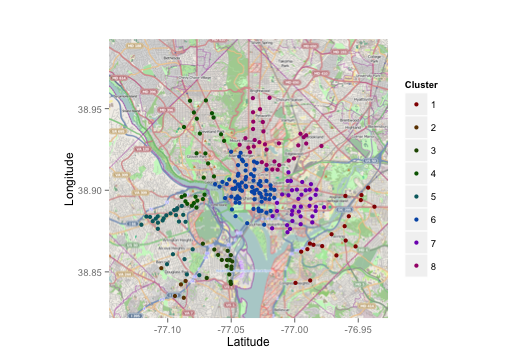
\includegraphics[scale = 0.2]{cluster_map.png}
\label{fig:cluster_map}
\end{figure}

We employ the clustering without knowledge of the range parameter; however, once we have the maximum likelihood estimate, $\hat{\theta}$, we will have an estimate of the range parameter, $\hat{\lambda}$.  The $k$-means clustering algorithm does not consider linear scaling of the distance function.  Therefore, if we simply re-estimate the clusters using the modified Euclidean distance, $\|{\bf z}_i - {\bf z}_j \| / \hat{\lambda}$, we will achieve the same partition.  However, we can now use the range estimate, to choose $k$ more  

\subsection{Parallel Estimation}

The block-diagonal approximation lightens the computational burden of the Monte-Carlo Simulations, as the conditional simulation of $\lambda$ condtional on $Y$ can be done in parallel.  However, the likelihood does not factorize by cluster under the current assumptions.  The approximate likelihood, $\hat{L} (\theta)$, does become a sum over independent clusters, but the assumption of common variance components means that estimation cannot be done in parallel across clusters.

If we assume that the variance components are distinct for each cluster, then we can estimate parameters separately for each cluster by exploiting variational independence.  This leads to additional computational savings as we can then parallelize the entire estimation procedure.  If the true variance components are identical for each cluster, then the estimated variance components for each cluster will be unbiased estimators.  Therefore, we only sacrifice slight losses in efficiency for gross gains in speed.  

\begin{algorithm}[!h]
\caption{Approximate Likelihood Algorithm} \label{applik_alg}
\begin{algorithmic}
\FOR{$i$ in stations}
\STATE $\mu_i \gets$ Fit marginal model $i$ 
\ENDFOR
\STATE Obtain initial estimate for $\sigma_0^2 = \text{mean} \{ \sigma_{0,j}^2\}$
\STATE Obtain initial estimate for $\sigma_1^2 = \sigma_2^2 = \sigma_0^2 / 2$
\STATE $U_1, U_2, \ldots U_k \gets$ cluster$(k, \text{stations})$
\FOR{$j$ in $1:k$}
\STATE $\theta_j \gets \text{ApproxCP} (Y_j, s, \theta_0)$ for Cluster $U_j$
\ENDFOR
\end{algorithmic}
\end{algorithm}

Given the approximate maximum likelihood estimate, $\theta$, we now turn our attention to estimating the desired quantities.

\section{Prediction}

For a particular station~$i$ at a particular time~$t$, we know the number of bikes at the station, $Y_i(t)$.  We are interested in estimation of the expected number of bikes at some future time point, $t+\delta$.  To answer the question of re-distribution, we also need to know the probability that the number of bikes reaches an extreme value in the time window $(t, t+\delta)$.  Therefore, assuming a maximum number of spots $\tau$, we want to estimate $\text{E} \left[ Y(t+ \delta) | Y(t) , \hat{\theta} \right]$ and $\text{P} [ Y(s) = 0 \text{ or } Y(s) = \tau \text{ for some } s \in (t, t+\delta) | Y(t), \hat{\theta} ]$.

Our block approximation from section~\ref{parallel_estimation}, allows estimation of both quantities to be done separately for each cluster.  Suppose station~$i$ sits inside cluster $U \subset \Omega$.

{\bf SECTION OUTLINE}
\begin{enumerate}
\item Simple : Station with data and neighboring stations
\item Add a new Station:   Need to infer the model for that station
\item Cluster Analysis
\item What about a new system?  Assume the covariates are okay, then we still need to do a cluster analysis
\end{enumerate}
\vspace{0.5cm}

\section{Online Learning: Algorithm and Prediction}

\vspace{0.25cm}
{\bf SECTION OUTLINE}
\begin{enumerate}
\item Want a manner to update paramaters in an online setting as the `latest numbers' provide the most updated solutions
\item We want to do this in a very simple way
\item Use the online algorithms and approximate block models
\end{enumerate}
\vspace{0.5cm}


\section{Experimental Results}

\vspace{0.25cm}

\subsection{Washington D.C. Bikeshare}
\vspace{0.25cm}
{\bf SECTION OUTLINE}
\begin{enumerate}
\item Explain the Complete Dataset
\item Include Maps
\item Explain how the `data' is common to Chicago given the layout of the city but it will not be common to other cities
\item 
\end{enumerate}
\vspace{0.5cm}

\subsection{Performance Indices}

\vspace{0.25cm}
{\bf SECTION OUTLINE}
\begin{enumerate}
\item How do we measure success?
\item We need good short term (`15 min' predictions) vs long term predictions of counts
\item We also want good prediction of the probability of being empty or full?
\item Need baseline and alternatives for comparison
\end{enumerate}
\vspace{0.5cm}

\section{Summary}


\end{document}
